\section{Implementasi}

Bagian ini akan menjelaskan tentang implementasi sistem kontrol adaptif secara terperinci.

\subsection{Batasan Implementasi}
Berikut adalah batasan yang ditetapkan dalam melakukan implementasi sistem kontrol adaptif.
\begin{enumerate}
    \item Semua batasan masalah dan konfigurasi yang telah dibahas pada bagian \ref{sec:batasan-masalah}.
    \item Komponen \textit{Metrics Fetcher} berjalan di proses lain dan diimplementasikan dalam \textit{script} yang berbeda dikarenakan bahasa Python memiliki kekurangan dalam penanganan \textit{multithreading}.
    \item Pertukaran data antara komponen \textit{Metrics Fetcher} dan \textit{Predictor} melalui stream file.
\end{enumerate}

\subsection{Kakas yang Digunakan}
Dalam melakukan implementasi ini diperlukan beberapa kakas, diantaranya adalah sebagai berikut.
\begin{enumerate}
    \item \textit{Docker}, \textit{Docker Desktop} dan \textit{Docker Desktop Kubernetes} untuk dipakai sebagai \textit{containerization} dan \textit{cluster} kubernetes lokal.
    \item Pandas dan Numpy untuk keperluan \textit{data processing} serta bentuk data untuk dikirimkan ke komponen lain serta model prediksi ARIMA.
    \item \textit{Kubernetes Python Client} untuk mengontrol \textit{cluster} kubernetes melalui kode Python.
    \item \textit{Pickle} untuk menyimpan model ARIMA sehingga persisten meskipun sistem di-\textit{restart}.
    \item \textit{Statsmodels} dan \textit{pmdarima} untuk membangun model ARIMA serta melakukan otomasi pencarian orde atau lebih dikenal sebagai Auto-ARIMA.
\end{enumerate}

\subsection{Persiapan \textit{Pods Elastic Search}}

Sebelum melakukan implementasi, diperlukan untuk menyalakan \textit{Pods Elastic Search}. Konfigurasi ini dilakukan dengan cara membuat \textit{file deployment} untuk \textit{pods Elastic Search} serta sebuah \textit{persistent volume claim} untuk tempat penyimpanan data. Sebagai contoh dan konfigurasi yang dipakai dalam membuat tugas akhir ini dapat dilihat pada lampiran \ref{appendix:cth-konfigurasi-es-pods}.

\subsection{Pengujian Komponen \textit{Metrics Fetcher}}

Pada bagian ini akan dijelaskan tentang tujuan, skenario, hasil, dan analisis dari pengujian komponen \textbf{\textit{Metrics Fetcher}}.

\subsubsection{Tujuan Pengujian}

Tujuan pengujian ini memastikan komponen \textbf{\textit{Metrics Fetcher}} dapat berjalan dengan baik dan menghasilkan data yang sesuai dengan ekspektasi.

\subsubsection{Skenario Pengujian}

Pengujian terhadap komponen \textbf{\textit{Metrics Fetcher}} dilakukan dengan beberapa skenario sebagai berikut serta ekspektasi dari pengujian yang dilakukan.
\begin{enumerate}
  \item \bfseries\textit{Elastic Search} sedang \textit{idle}.\normalfont

        Data yang diminta dari \textit{Node Stats API} diekspektasikan relatif statis dan berhasil diletakkan pada \textit{stream file}.
  \item \bfseries\textit{Elastic Search} sedang digunakan untuk melakukan operasi penambahan data.\normalfont

        Data yang diminta dari \textit{Node Stats API} seharusnya relatif berubah terutama pada aspek \textit{throughput} operasi \textit{index} dan \textit{bulk}. Lalu, data tersebut diekspektasikan berhasil diletakkan pada \textit{stream file}.

  \item \bfseries\textit{Elastic Search} sedang digunakan untuk melakukan operasi pencarian data.\normalfont

        Data yang diminta dari \textit{Node Stats API} seharusnya relatif berubah terutama pada aspek \textit{throughput} operasi \textit{query} dan \textit{fetch}. Lalu, data tersebut diekspektasikan berhasil diletakkan pada \textit{stream file}.
\end{enumerate}

\subsubsection{Hasil Pengujian dan Analisis}

Hasil untuk skenario 1 dapat dilihat pada gambar \ref{fig:mf-1}. Data yang ditarik sudah relatif statis untuk semua aspek dan berhasil diletakkan pada \textit{stream file}. Untuk skenario 2, dapat dilihat pada gambar \ref{fig:mf-2}. Data yang ditarik sudah mengalami perubahan pada operasi \textit{index} dan \textit{bulk} serta berhasil diletakkan pada \textit{stream file}. Terakhir, skenario 3, dapat dilihat pada gambar \ref{fig:mf-3}. Data yang ditarik sudah mengalami perubahan pada operasi \textit{query} dan \textit{fetch} serta berhasil diletakkan pada \textit{stream file}.

\begin{figure}[h]
  \centering
  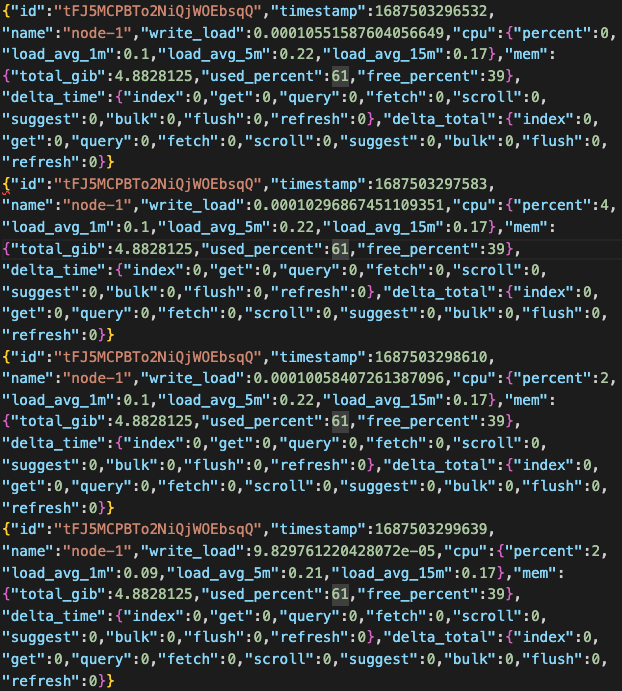
\includegraphics[width=0.8\textwidth]{chapter-4/mf-1.png}
  \caption{Hasil Pengujian Komponen \textit{Metrics Fetcher} Skenario 1}
  \label{fig:mf-1}
\end{figure}

\begin{figure}[h]
  \centering
  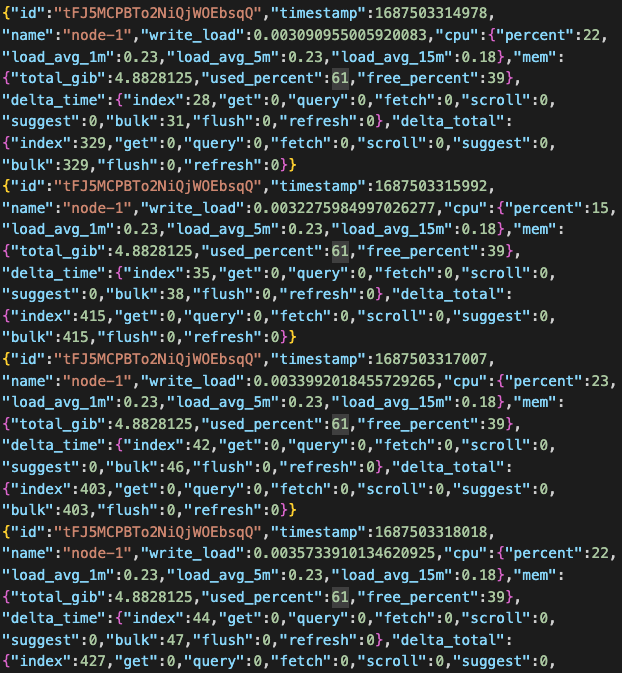
\includegraphics[width=0.8\textwidth]{chapter-4/mf-2.png}
  \caption{Hasil Pengujian Komponen \textit{Metrics Fetcher} Skenario 2}
  \label{fig:mf-2}
\end{figure}

\begin{figure}[h]
  \centering
  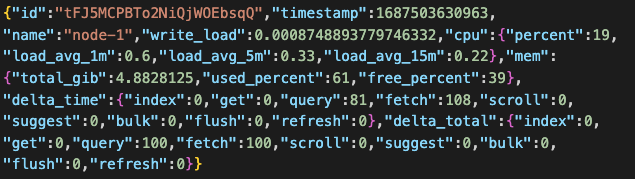
\includegraphics[width=0.8\textwidth]{chapter-4/mf-3.png}
  \caption{Hasil Pengujian Komponen \textit{Metrics Fetcher} Skenario 3}
  \label{fig:mf-3}
\end{figure}

Pengujian komponen \textbf{\textit{Metrics Fetcher}} sudah sesuai ekspektasi dan dapat dilanjutkan ke pengujian komponen lainnya.
\subsubsection{Komponen \textbf{\textit{Predictor}}}
Komponen \textbf{\textit{Predictor}} dirancangkan terdiri dari 3 buah kelas, yaitu sebagai berikut.
\begin{enumerate}
    \item \textbf{\textit{Predict Component}}
    
    Kelas ini berfungsi untuk menyimpan sebuah model ARIMA untuk sebuah variabel. Kelas ini memanfaatkan kakas pandas, statsmodels dan pmdarima untuk melakukan tanggung jawabnya.

    \item \textbf{\textit{Predict Component Factory}}
    
    Kelas ini berfungsi untuk membuat objek \textbf{\textit{Predict Component}} sebanyak variabel yang ada. 

    \item \textbf{\textit{Predict Component Storage}}
    
    Kelas ini berfungsi sebagai aggregator objek \textbf{\textit{Predict Component}} yang telah dibuat oleh \textbf{\textit{Predict Component Factory}}. Kelas ini juga berfungsi untuk meneruskan sebuah aksi kepada semua objek \textbf{\textit{Predict Component}} yang ada. Contohnya, dengan memanggil \textit{forecast} atau \textit{update data}, maka operasi akan diteruskan ke semua objek \textbf{\textit{Predict Component}}.

\end{enumerate}

\begin{figure}[h]
    \centering
    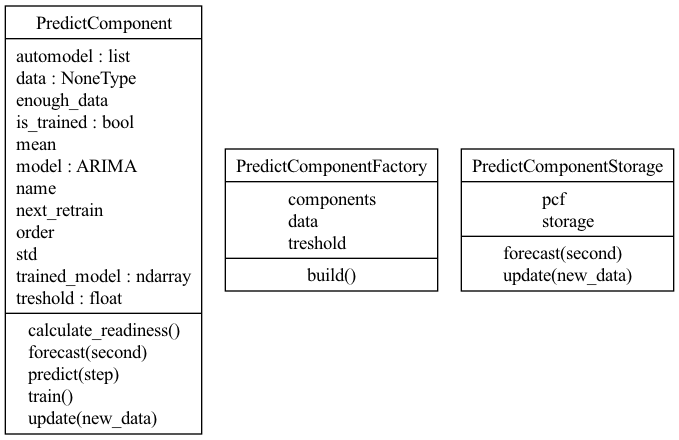
\includegraphics[width=0.8\textwidth]{chapter-4/predictor.png}
    \caption{Spesifikasi Kelas Penyusun Komponen \textit{Predictor}}
    \label{fig:predictor-spek}
\end{figure}

Secara umum, spesifikasi kelas bisa dilihat pada gambar \ref{fig:predictor-spek}. Kelas \textbf{\textit{Predict Component Storage}} akan membutuhkan \textbf{\textit{Predict Component Factory}} untuk membangun semua \textbf{\textit{Predict Component}} untuk setiap variabel yang ada. Setelah itu, terdapat operasi seperti meneruskan penambahan data serta meminta data prediksi ke setiap \textbf{\textit{Predict Component}}. Kelas ini akan digunakan oleh komponen \textbf{\textit{Flexible Control}} untuk lebih lanjutnya.
\subsubsection{Komponen \textbf{\textit{Rule Manager}}}
Komponen \textbf{\textit{Rule Manager}} dirancangkan melakukan parsing terhadap file \textit{rule} yang telah diisi oleh pengguna serta menjadi aggregator untuk melakukan pengecekan \textit{rule} yang berlangsung serta memberi informasi data prediksi kapan saja yang dibutuhkan untuk melakukan pengecekan. Parsing komponen ini menggunakan format csv dan kondisi diekspresikan dengan sintaks python. Komponen akan mengonstruksi objek \textbf{\textit{Rule}} yang akan digunakan oleh komponen \textbf{\textit{Flexible Control}}. Spesifikasi dari kedua kelas tersebut dapat dilihat pada gambar \ref{fig:rule-spek}.

\begin{figure}[h]
    \centering
    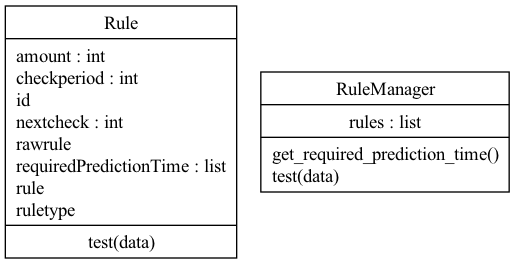
\includegraphics[width=0.8\textwidth]{chapter-4/rule.png}
    \caption{Spesifikasi Kelas Penyusun Komponen \textit{Rule Manager}}
    \label{fig:rule-spek}
\end{figure}

Sebuah \textit{rule} memiliki fungsi sebagai berikut.
\begin{enumerate}
    \item Memiliki sebuah kondisi yang akan dievaluasi dengan data prediksi pada waktu prediksi yang diinginkan. Contoh: kondisi \textit{throughput} untuk operasi X untuk 1 menit kedepan dan 5 menit kedepan lebih dari 1s, maka tingkatkan prosesor sebanyak 500m.
    \item Memiliki jumlah serta target kategori untuk diubah, dalam kasus ini pilihannya memori atau prosesor.
    \item Satuan untuk perubahan memori adalah dalam \textit{Mebibyte} atau MiB. Sedangkan untuk prosesor dalam satuan mili atau m.
    \item Sebuah \textit{rule} memiliki periode pengecekan sehingga tidak akan dicek secara terus menerus yang menyebabkan perubahan alokasi sumber daya terlalu cepat. Periode pengecekan dibuat dalam satuan sekon.
\end{enumerate}
\subsection{Komponen \textit{Resource Controller}}

Seperti yang sudah dirancangkan sebelumnya, kelas ini menggunakan \textit{Kubernetes Client API} untuk mengubah alokasi sumber daya. Diimplementasikan dengan sistem antrian, sehingga jika sejumlah rule aktif secara bersamaan, maka akan dijalankan secara berurutan. Terdapat sebuah fungsi \textit{tick} yang akan berfungsi untuk mengeksekusi antrian. Contoh simpanan file antrian dapat dilihat pada gambar \ref{fig:ex-queue-rc}. File tersebut menyimpan status alokasi sumber daya pada saat itu, kapan melakukan perubahan pada antrian berikutnya dalam waktu UNIX dan antrian yang akan dieksekusi satu per satu.

\begin{figure}[h]
    \centering
    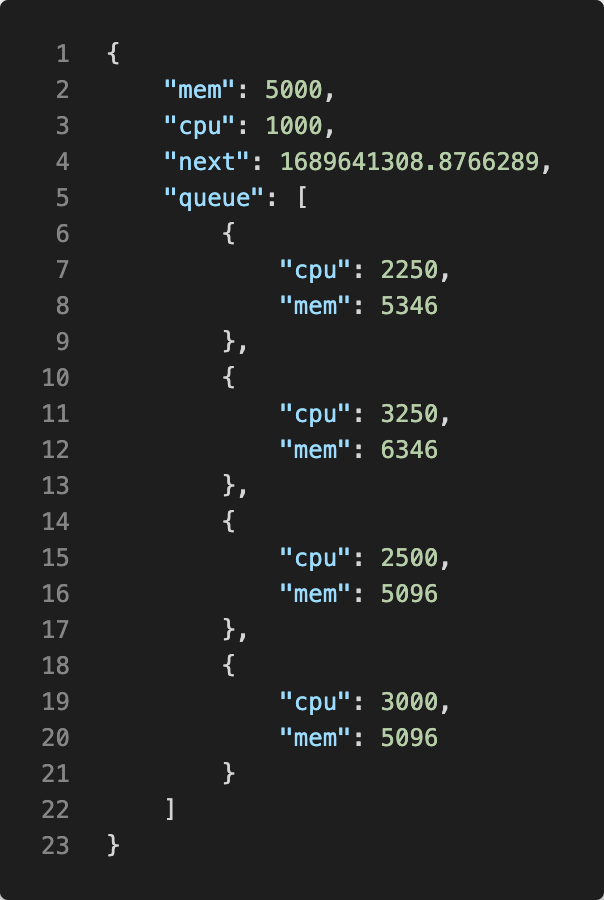
\includegraphics[width=0.45\textwidth]{chapter-4/rc-queue-ex.png}
    \caption{Contoh File Antrian Pengubahan Alokasi}
    \label{fig:ex-queue-rc}
\end{figure}

% TODO CONTOH SISTEM ANTRIAN
% \subsection{Pengujian Sistem \textit{Flexible Control}}

Pada bagian ini akan dijelaskan tentang tujuan, skenario, hasil, dan analisis dari pengujian sistem sekaligus komponen \textbf{\textit{Flexible Control}}.

\subsubsection{Tujuan Pengujian}

Tujuan pengujian ini memastikan sistem \textbf{\textit{Flexible Control}} dapat berjalan dengan baik dan menghasilkan perilaku yang sesuai.

\subsubsection{Skenario Pengujian}

Pengujian terhadap komponen \textbf{\textit{Flexible Control}} dilakukan dengan beberapa skenario sebagai berikut serta ekspektasi dari pengujian yang dilakukan.
\begin{enumerate}
  \item \bfseries Sebuah \textit{rule} memenuhi kondisi untuk mengubah alokasi prosesor.\normalfont

        Prosesor akan berubah jumlahnya sesuai dengan \textit{rule} yang memenuhi kondisi. Perubahan pada spesifikasi \textit{pods} juga diekspektasikan mengikuti.

  \item \bfseries Sebuah \textit{rule} memenuhi kondisi untuk mengubah alokasi memori.\normalfont

        Prosesor akan berubah jumlahnya sesuai dengan \textit{rule} yang memenuhi kondisi. Perubahan pada spesifikasi \textit{pods} juga diekspektasikan mengikuti. Memory Used Percent akan menurun karena penambahan yang terjadi.
\end{enumerate}

\subsubsection{Hasil Pengujian dan Analisis}

Pengujian akan dilakukan dengan \textit{file rule} yang dapat dilihat pada gambar \ref{fig:ac-rule}. Terdapat dua buah \textit{rule} yang akan diuraikan sebagai berikut.

\begin{enumerate}
  \item Jika \textit{load average 1m} pada 10 detik kedepan diprediksikan diatas 0 maka akan ditambah alokasi prosesor sebesar 1000m atau sejumlah 1. Kondisi dari \textit{rule} sengaja dibuat seperti itu agar rule pasti terpenuhi.
  \item Jika \textit{memory used percent} pada 5 dan 10 detik kedepan diprediksikan diatas 60 maka akan ditambah alokasi memori sebesar 2048 mebibyte atau sejumlah 2 gibibyte (Gi). Kondisi dari \textit{rule} sengaja dibuat seperti itu agar rule pasti terpenuhi.
\end{enumerate}

Hasil dari pengujian skenario kedua dapat dilihat pada gambar \ref{fig:ac-mem}. Dan perubahan terhadap spesifikasi pods dapat dilihat pada gambar \ref{fig:ac-mem-kube}. Perubahan juga terjadi pada \textit{memory used percent} pada \textit{stream file} atau data yang ditarik oleh komponen \textbf{\textit{Metrics Fetcher}} dapat dilihat pada gambar \ref{fig:ac-mf-turun}.
Diikuti dengan hasil dari pengujian skenario pertama dapat dilihat pada gambar \ref{fig:ac-cpu}. Dapat dilihat bahwa prosesor berubah sesuai dengan ekspektasi. Perubahan pada spesifikasi \textit{pods} juga mengikuti perubahan prosesor yang dapat dilihat pada gambar \ref{fig:ac-cpu-kube}.

\begin{figure}[h]
  \centering
  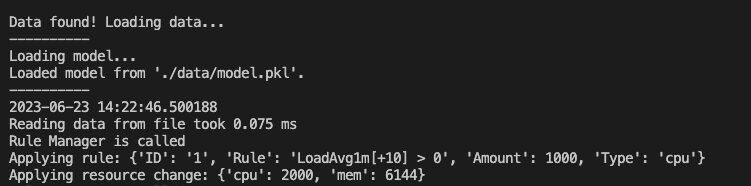
\includegraphics[width=0.8\textwidth]{chapter-4/ac-cpu.png}
  \caption{Hasil Pengujian Komponen \textit{Flexible Control} Skenario 1: Perubahan Prosesor}
  \label{fig:ac-cpu}
\end{figure}

\begin{figure}[h]
  \centering
  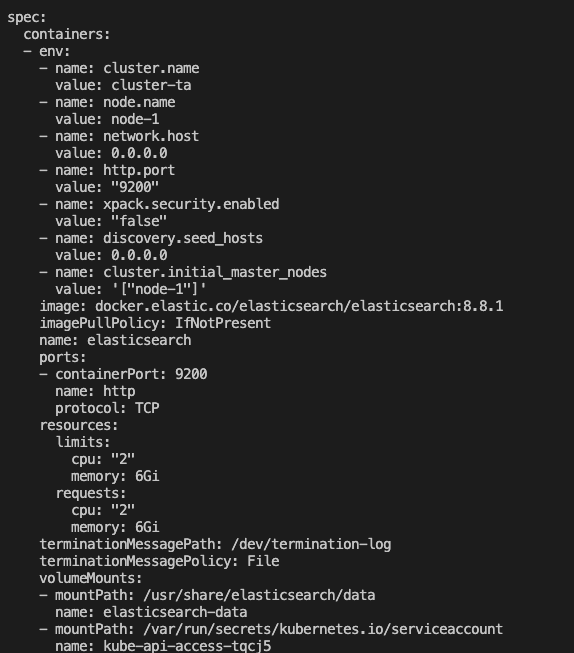
\includegraphics[width=0.8\textwidth]{chapter-4/ac-cpu-kube.png}
  \caption{Hasil Pengujian Komponen \textit{Flexible Control} Skenario 1: Perubahan Spesifikasi Kubernetes}
  \label{fig:ac-cpu-kube}
\end{figure}

\begin{figure}[h]
  \centering
  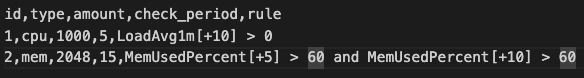
\includegraphics[width=0.8\textwidth]{chapter-4/ac-rule.png}
  \caption{File Rule untuk Pengujian Komponen \textit{Flexible Control}}
  \label{fig:ac-rule}
\end{figure}

\begin{figure}[h]
  \centering
  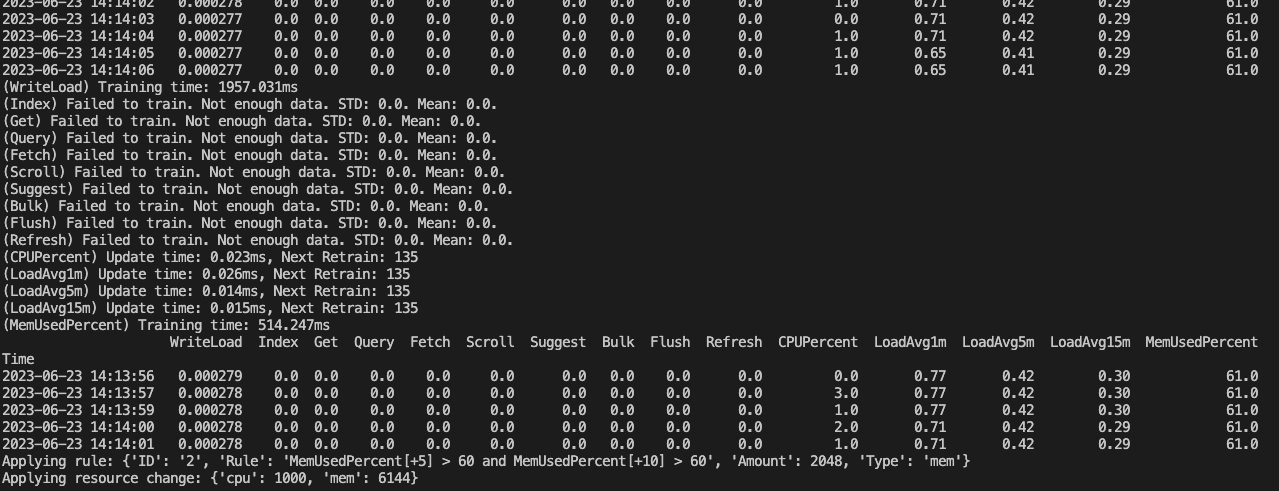
\includegraphics[width=1\textwidth]{chapter-4/ac-mem.png}
  \caption{Hasil Pengujian Komponen \textit{Flexible Control} Skenario 2: Perubahan Memori}
  \label{fig:ac-mem}
\end{figure}

\begin{figure}[h]
  \centering
  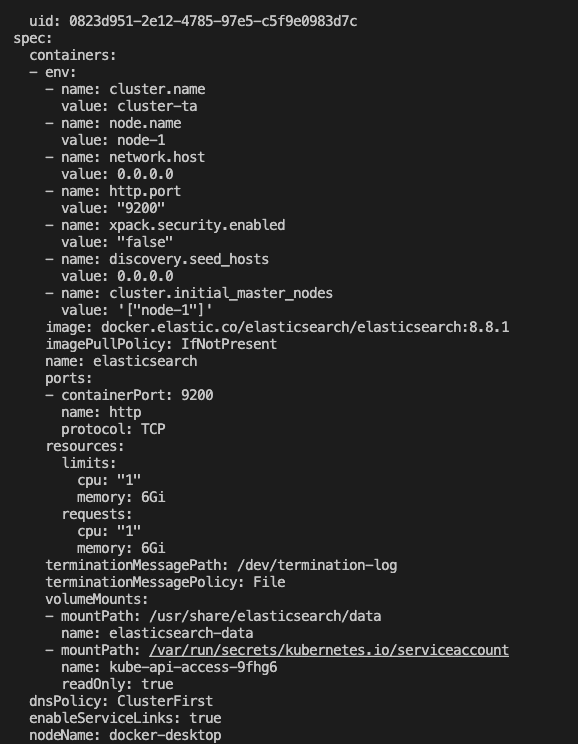
\includegraphics[width=0.8\textwidth]{chapter-4/ac-mem-kube.png}
  \caption{Hasil Pengujian Komponen \textit{Flexible Control} Skenario 2: Perubahan Spesifikasi Kubernetes}
  \label{fig:ac-mem-kube}
\end{figure}

\begin{figure}[h]
  \centering
  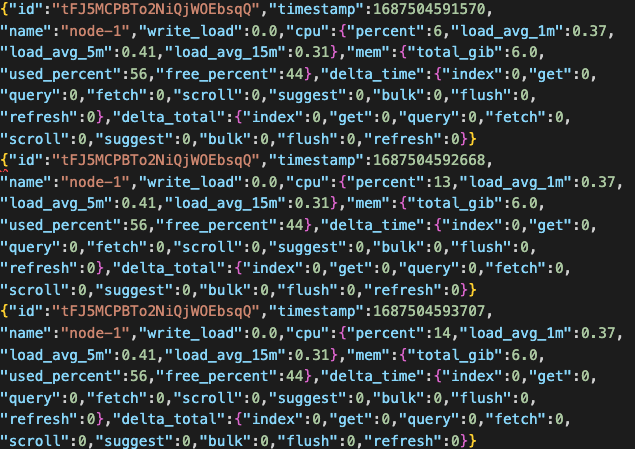
\includegraphics[width=0.8\textwidth]{chapter-4/ac-mf-turun.png}
  \caption{Hasil Pengujian Komponen \textit{Flexible Control} Skenario 2: Perubahan Memory Used Percent pada \textit{stream file}}
  \label{fig:ac-mf-turun}
\end{figure}

Pengujian komponen \textbf{\textit{Flexible Control}} sudah sesuai ekspektasi dan sistem dapat berjalan dengan baik.
\subsection{Komponen Pendukung: Konfigurasi dan Utilitas}
\label{sec:komponen-pendukung}

Seperti yang sudah dijelaskan sebelumnya, terdapat konfigurasi yang dapat mengatur sistem. Konfigurasi yang dapat diatur dapat dilihat pada gambar \ref{fig:config-spek}.

\begin{figure}[ht]
  \centering
  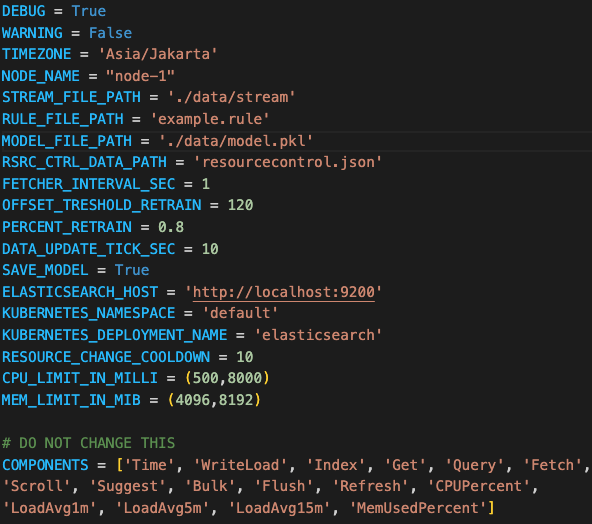
\includegraphics[width=0.8\textwidth]{chapter-4/config.png}
  \caption{Konfigurasi \textit{Flexible Control}}
  \label{fig:config-spek}
\end{figure}

Setiap konfigurasi tersebut mengatur perilaku dari sistem. Untuk setiap konfigurasinya, berikut adalah penjelasannya.

\begin{enumerate}
  \item \textbf{\textit{Debug}} dan \textbf{\textit{Warning}}

        Kedua \textit{flag} ini adalah untuk mematikan dan menyalakan pesan \textit{debug} dan \textit{warning}. Jika \textit{debug} dimatikan, maka program tidak akan mengirimkan pesan apapun selama berjalan.

  \item \textbf{\textit{Timezone}}

        Flag ini bertujuan untuk mengubah zona waktu yang digunakan oleh pandas karena data yang didapatkan dari \textit{Elastic Search} adalah berupa unix time sehingga akan dibaca secara \textit{default} menjadi UTC saat dikonversi.

  \item \textbf{\textit{Node Name}}, \textbf{\textit{Namespace}} dan \textbf{\textit{Deployment Name}}

        \textbf{\textit{Node Name}} adalah nama \textit{node} yang telah dikonfigurasi pada \textit{pods Elastic Search}. Nama harus sesuai karena \textbf{\textit{Metrics Fetcher}} akan mencari data untuk node dengan nama tersebut. Sedangkan, \textbf{\textit{Namespace}} dan \textbf{\textit{Deployment Name}} berkaitan dengan \textit{namespace} dan \textit{deployment Elasticsearch} dengan Kubernetes.

  \item \textbf{\textit{Elasticsearch Host}}

        \textit{Flag} ini berisikan target \textit{host} dari \textit{Elasticsearch}. Bertindak sebagai \textit{Base URL} untuk mengakses API \textit{Elastic Search}.

  \item \textbf{\textit{CPU Limit}} dan \textbf{\textit{Memory Limit}}

        Kedua limit ini digunakan untuk \textbf{\textit{Resource Controller}} mengubah alokasi sumber daya. \textit{Flag} ini berisikan \textit{tuple} dengan dua buah angka yang berguna sebagai batas bawah dan batas atas dari sumber daya bersangkutan. Satuan yang digunakan untuk prosesor adalah mili (m) sedangkan untuk memori adalah \textit{mebibyte} (MiB). Kedua batas ini bersifat inklusif.

  \item \textbf{\textit{File Path}}

        Seperti namanya, konfigurasi yang berkaitan dengan \textit{file path} berfungsi untuk mengatur tata letak file yang akan dibuat/dibaca oleh sistem.

  \item \textbf{\textit{Fetcher Interval}}, \textbf{\textit{Resource Change Cooldown}} dan \textbf{\textit{Data Update Tick Second}}

        \textbf{\textit{Fetcher Interval}} adalah interval komponen \textbf{\textit{Metrics Fetcher}} melakukan penarikan data. Lalu, \textbf{\textit{Resource Change Cooldown}} adalah waktu yang diperlukan oleh \textbf{\textit{Resource Controller}} untuk menunggu sebelum melakukan perubahan sumber daya. Terakhir, \textbf{\textit{Data Update Tick Second}} adalah interval yang digunakan oleh \textbf{\textit{Flexible Control}} untuk melakukan pembacaan data dari \textit{stream file}. \textbf{\textit{Data Update Tick Second}} harus lebih besar sama dengan \textbf{\textit{Fetcher Interval}} agar efisien. Satuan yang digunakan oleh ketiga \textit{flag} tersebut adalah detik.

  \item \textbf{\textit{Save Model}}

        \textit{Flag} ini berfungsi untuk mematikan penyimpanan model setiap kali model berubah. Jika \textit{flag} ini tidak dinyalakan, maka setiap kali sistem melakukan \textit{restart}, model prediksi akan diulang dari kosong.

  \item \textbf{\textit{Offset Treshold Retrain}} dan \textbf{\textit{Percent Retrain}}

        Dalam melakukan penambahan data, tidak setiap saat model akan di-\textit{retrain}. Saat tidak di-\textit{retrain}, model prediksi hanya melakukan update yang jauh lebih cepat namun tidak terlalu akurat. Terdapat sebuah angka yang akan menentukan kapan model harus di-\textit{retrain}. Hal ini diperlukan karena melakukan \textit{retrain} membutuhkan waktu yang lama terutama saat data sudah sangat besar. \textbf{\textit{Offset Treshold Retrain}} adalah angka yang menentukan kapan model harus di-\textit{retrain} berdasarkan jumlah data fixed. Sedangkan, \textbf{\textit{Percent Retrain}} adalah angka yang menentukan kapan model harus di-\textit{retrain} berdasarkan persentase jumlah data saat itu. Dengan persamaan \ref{eq:retrain-time}, \textbf{\textit{Offset Treshold Retrain}} adalah variable $c$ dan \textbf{\textit{Percent Retrain}} adalah variable $p$.
\end{enumerate}

Terdapat juga fungsi-fungsi utilitas yang akan membantu komponen-komponen yang telah dijelaskan sebelumnya, spesifikasi utilitas bisa dilihat pada gambar \ref{fig:util-spek}. Untuk setiap fungsinya, berikut adalah kegunaannya.

\begin{enumerate}
  \item \textbf{\textit{Save Model}}

        Fungsi ini akan menyimpan model yang telah dilatih ke dalam sebuah file. Digunakan kakas \textit{pickle} untuk melakukan hal ini.

  \item \textbf{\textit{Load Model}}

        Fungsi ini akan memuat model yang telah dilatih dari sebuah file. Digunakan kakas \textit{pickle} untuk melakukan hal ini.

  \item \textbf{\textit{Timings}}

        Fungsi adalah abstraksi untuk menghitung waktu eksekusi. Digunakan fungsi sebagai \textit{return value} agar lebih rapih ketika diperlukan banyak penghitungan waktu eksekusi.

  \item \textbf{\textit{Printd}}

        Fungsi ini hanyalah \textit{wrapper} dari fungsi \textit{print} pada Python untuk mengikuti aturan konfigurasi.

  \item \textbf{\textit{Read From File}}

        Fungsi ini digunakan untuk membaca \textit{stream file}. Fungsi ini digunakan oleh komponen \textbf{\textit{Flexible Control}} untuk membaca secara periodik, mentranformasikan dan mengirimkan data ke \textbf{\textit{Predict Component Storage}}.

  \item \textbf{\textit{To Vector}}

        Fungsi ini adalah fungsi transformasi format JSON (\textit{Java Syntax Object Notation}) yang ditulis ke \textit{stream file} menjadi sebuah \textit{numpy array} yang akan digunakan untuk membuat \textit{pandas dataframe}.

  \item \textbf{\textit{Create Dataframe}}

        Seperti namanya, fungsi ini membuat dataframe dari data yang telah dibaca dari \textit{stream file} dan sudah ditransformasikan dengan fungsi \textbf{\textit{to vector}}.

  \item \textbf{\textit{Extract Number From String}}

        Fungsi ini memanfaatkan regex untuk mengambil angka dari sebuah string.
\end{enumerate}

\begin{figure}[ht]
  \centering
  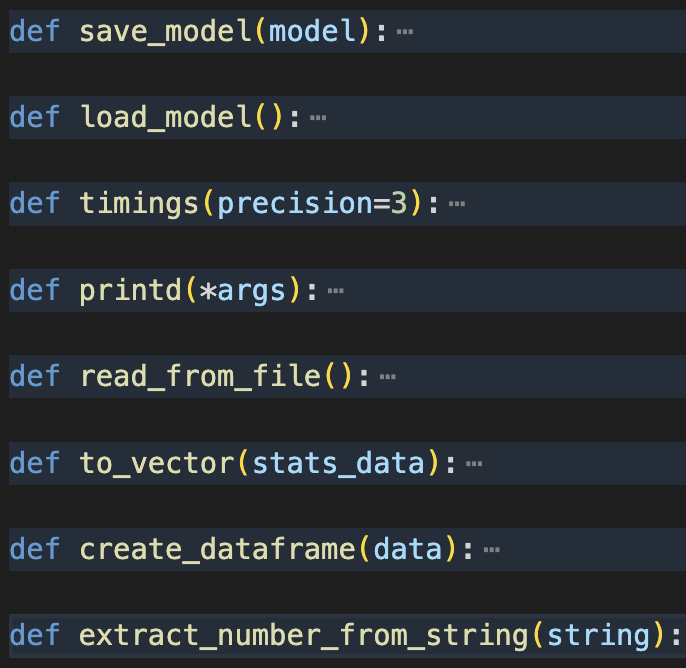
\includegraphics[width=0.6\textwidth]{chapter-4/utils.png}
  \caption{Spesifikasi Fungsi Utilitas Pendukung}
  \label{fig:util-spek}
\end{figure}

\subsection{Penggunaan untuk \textit{Pods} dengan Aplikasi Lain}

Sistem yang diimplementasikan juga dapat digunakan untuk pods lainnya. Tentunya dengan mengubah konfigurasi serta membuat \textbf{\textit{Metrics Fetcher}} khusus untuk aplikasi tersebut. Berikut adalah \textit{requirement} untuk dapat digunakan pada \textit{pods} lain.

\begin{enumerate}
    \item Aplikasi tersebut harus memiliki \textit{metrics} yang dapat diambil melalui suatu API, dapat berbentuk HTTP, GRPC atau yang lainnya. \label{item:requirement-general-1}
    \item Aplikasi harus bisa mempunyai komponen untuk menghitung \textit{throuhgput} untuk setiap operasinya. \label{item:requirement-general-2}
\end{enumerate}

Ketika poin \ref{item:requirement-general-1} dan \ref{item:requirement-general-2} sudah terpenuhi, maka langkah-langkah yang harus dilakukan adalah sebagai berikut.

\begin{enumerate}
    \item Membuat komponen \textbf{\textit{Metrics Fetcher}} yang baru untuk aplikasi tersebut.
        
        Dalam melakukan hal ini, transformasi sebaiknya diusahakan disesuaikan dengan struktur data yang sudah ada. Namun, jika ingin mengubah, maka harus melakukan pengubahan ekstra pada fungsi pemetaan \textit{metrics} yang ada pada komponen \textbf{\textit{Predictor}}.
    \item Menyesuaikan konfigurasi dan fungsi pemetaan komponen \textbf{\textit{Predictor}}.

        Tentunya, nama operasi akan berbeda serta detil-detil utilisasi umum akan berbeda sehingga diperlukan untuk mengubah dan menyesuaikan pada file konfigurasi.

    \item Mengubah \textit{label selector kubernetes} pada komponen \textbf{\textit{Resource Controller}}

        Karena sebelumnya dispesifikan ke aplikasi \textit{Elastic Search}, akibatnya, untuk mengubah ke aplikasi lain, perlu melakukan pengubahan \textit{label selector}.
\end{enumerate}

Setelah melakukan pengubahan tersebut, sistem sudah dapat digunakan untuk aplikasi lainnya.